\documentclass[12pt]{article}
\pagenumbering{arabic}
\pdfpagewidth 8.5in
\pdfpageheight 11in
\setlength\topmargin{0in}
\setlength\headheight{0in}
\setlength\headsep{0in}
\setlength\textheight{9.0in}
\setlength\textwidth{6.5in}
\setlength\oddsidemargin{0in}
\setlength\evensidemargin{0in}
\setlength\parindent{0.25in}
\setlength\parskip{0.25in}
\parskip 0.0pt
\usepackage[utf8]{inputenc}
\usepackage[english]{babel}
\usepackage{amsmath}
\usepackage{amsfonts}
\usepackage{amssymb}
\usepackage{amsbsy}
\usepackage{setspace}
\usepackage{graphicx}
\usepackage{tabularx,ragged2e,booktabs,caption}
\usepackage{float}
\usepackage{dcolumn}
\usepackage{natbib}
\usepackage{subfigure}
\usepackage{xcolor}
\usepackage{hyperref}

\begin{document}  


\begin{titlepage}




\title{Let Them Tweet Cake: Estimating Public Dissent and Political Stability using Twitter}



\author{Ethan Spangler\thanks{Corresponding Author. Email: {\href{mailto:eospangler@gmail.com}{eospangler@gmail.com}}} \\ %; Tel: 801-458-9923; Washington State University School of Economic Sciences Hulbert Hall 101, Pullman, WA 99164, United States}  \\
Ben Smith\thanks{Email: {\href{mailto:bosmith@unomaha.edu}{bosmith@unomaha.edu}}; University of Nebraska-Omaha Mammel Hall, Suite 332, 6708 Pine Street, Omaha, NE 68182, United States}}



\date{\today}

\maketitle

\begin{abstract}
\noindent Traditional methods of estimating political stability have been unreliable, unable to adapt quickly to the realities on the ground. Thus it is the goal of this paper to create a new measure of political stability, one with a firm theoretical foundation and that utilizes advances in social media. Twitter, a micro-blogging website, allows users to post short messages (tweets) that can be viewed and shared by other users, creating a vast network of freely and easily observable information. We collect tweets from citizens containing specified words or phrases voicing dissatisfaction with their government. Collected tweets are then scored and aggregated; forming the basis of the measure of public dissent. Combining these estimates of dissent with macroeconomic data of the country within an established theoretical framework, creates an overall estimation of a country's political stability. A case study on Canada and Kenya provides proof of concept.
\end{abstract}

\noindent \textit{Keywords}: Twitter, Political Stability, Dissent \\

\noindent \textit{JEL Code}: C80, O57, P16




\end{titlepage}





\begin{spacing}{1.5}

\section*{Introduction}

The importance of political stability is well established and can affect all aspects of an economy (Kaufmann et al. 1999b) and substantially impede economic growth (Alesina and Perotti, 1996; Jong-A-Pin, 2009; Aisen and Veiga, 2013). Additionally, there is a propensity for a country's political stability issues to leak beyond its borders (Murdoch and Sandler, 2002), negatively affecting neighboring nations' stability and creating large scale welfare implications. However, despite its significance, measurement of political stability has remained underdeveloped. 

As demonstrated by the recent uprisings in the Middle East, Thailand, and Ukraine; large scale political changes are difficult to predict. The three commonly used measures of political stability are Political Risk Services (PRS), the Business Environment Risk Intelligence Index (BERI), and the Economist Intelligence Unit (EIU). Each of these indexes combine political, financial, and economic factors to assess a nation's political stability (Howell, 1998). The financial and economic portions are predominately based on quantitative data (foreign debt, inflation, GDP per capita, etc) while political factors are more qualitative. 

Political factors for each index are determined and scored by panels of experts (Howell, 1998). These experts are usually former diplomats, scholars, and other suitably qualified individuals. While these teams of experts can be quite large and knowledgeable, it is still a relatively small group of people trying to assess an entire nation. Additionally these experts lack a clear theoretical foundation for their decisions. 

Since political factors compose 33-66\% of each index (Howell, 1998), if these experts are somehow misinformed the validity of the index could be greatly affected. In turn this potential bias would affect all research based on these indexes. Additionally, Tetlock (2005) shows that political forecasts based on expert opinion are only marginally better than random chance. It becomes quite apparent that a new method of assessing political stability is needed.  

To highlight the issue of why a more robust measure of political stability is needed let us examine some contemporary examples and their related political stability analysis. The October 2005 PRS report on Thailand said ``unrest is not expected to threaten general stability, nor intensify to the point of endangering the [Thai Rak Thai Party's (TRT)] dominant political position...the chances of the TRT being forced from power at any point during the five year forecast period are slim..." (PRS 2006, p. 40). Less than a year later a military coup ousted the Prime Minister Shinawatra and outlawed his TRT party, and began a period of political strife that continues to plague Thailand. The PRS report on Ukraine published October 2012, stated that ``a repeat of the Orange Revolution...is unlikely." and ``Ukrainians are disillusioned but in general they possess little appetite for protest." (PRS 2013, p. 11). Mass protests began in November 2013 and by February 2014 the Yanukovych regime had fallen. The PRS report on Tunisia, published October 2010, called Tunisia an ``oasis of stability" (PRS 2011, p. 3) and postulated a 85\% probability that Tunisian dictator Ben Ali would retain power for the next 18 months. By January 2011, mass protests and revolt resulted in the dissolution of the ruling RCD party, the exile of Ben Ali to Saudi Arabia, and the establishment of an interim government. While it may be easy to critique these forecasts with the benefit of hindsight, these examples highlight the inherent difficulty in predicting something as opaque and complex as political stability.\footnote{It should be noted that PRS publishes monthly reports on its surveyed countries but those are only available to its subscribers.} 

A shared limitation of previous political stability measurements was a lack of both a theoretical framework and quality data. Thankfully, advancements in both areas have arisen that substantially mitigate these issues. Spangler and Smith (2017) establish a theoretical framework for understanding political stability. They base their theory on the dynamic interactions of a government and its citizens. Regarding data, the spread of social media platforms such as Twitter and development of text analysis techniques means that researchers can tap into the zeitgeist of a population.

In this paper we use online public dissent against a government as a basis for examining a country's political stability. Whereas previous measures of political stability relied on expert opinion, polling, or other traditional methodology; this paper develops a measure of political stability based on data collected from Twitter. The following sections of this paper will review literature concerning measuring political stability and other relevant topics, theoretical model, explanation of the methodology employed in this paper, proof of concept case studies using Canada and Kenya, and finally conclusion. 

\section*{Related Literature}   

We have already discussed the dominant methods for measuring political stability (Howell 1998) and their potential flaws, but there are other methods that need to be addressed. Kaufmann et al. (1999a) proposes using `aggregate governance indicators' which combines hundreds of different variables and indicators (including those built by PRS, BERI, and EUI) together to evaluate several factors of governmental quality to get the most out of available data. Jong-A-Pin (2009) uses a similar multi-dimensional approach to evaluate the economic impact of political stability. This approach does work to smooth out some of the issues of a single indicator but ultimately Kaufmann et al. concludes that contemporary methods ``point to the inadequacy of existing governance measures." (Kaufmann et al., 1999a p. 31). Other methods of evaluating government effectiveness rely on crowd sourcing, polling, and surveying; but all have their own limitations. 

Ungar et al. (2012) relies on expert opinion, but instead of just a few experts Ungar et al. employ thousands, using a mixture of crowd sourcing and simplification of complex issues. Ungar et al.'s approach works by having their army (over 2000 individuals) of forecasters assign probability estimates to specific events happening within a given time (Q:``Will Julius Caesar cease power before March 15\textsuperscript{th}?", A: Yes, 42\% probability.), updating their predictions as needed before the deadline. Finally, all predictions are combined to form a single aggregate forecast of the event. 

Ungar et al.'s method, and prediction markets in general, are extremely effective in harnessing the wisdom of crowds, but at the same time they are hamstrung by the simplifications needed in order to harness that wisdom. They work best when asking the crowd simple questions, which may not capture all the nuances and complexities necessary to understand an issue, especially when attempting to gauge a country's overall political stability. Additionally, in dealing with esoteric issues, there might only be a few experts with area knowledge, which leaves this method vulnerable to the same problems as described earlier (Tetlock, 2005). Finally, maintaining and incentivizing a vast number of forecasters is likely to be very costly and time intensive, as one must wait for forecasters to make and adjust their judgements. 

Polling and surveying provide flexible formats for assessment and when implemented properly can be effective. Paired with demographic information, they can also be quite focused. Unfortunately effective polling and surveying is costly and time consuming. There are also unique issue to polling and surveying that are difficult for researchers to overcome. The biggest hurdle is one of honesty since respondents often have little incentive to be honest, to varying degrees of malevolence. For instance, polls and surveys are susceptible to the `social desirability bias', wherein respondents have a tendency to provide what they perceive to be the socially acceptable answer to questions (Setphens-Davidowitz, 2017). This especially could be a problem if someone is being asked about popular government entities or policies they are in the opposition to. 

The issue is further intensified by the fact that many places where accurate measurement of political stability is most needed, might also be places where honest public speech is not safe. According to Freedom House (2017), of the 195 countries evaluated, only 44\% were regarded as `free' in regards to political rights. This means that in most countries a person might be unwilling to provide their honest thoughts to a stranger asking about their government. On the other extreme, respondents may provide strategic answers with the intent of influencing potential policy that may be based on poll results, biasing results (Morgan and Stocken, 2008). Finally, results could be biased because respondents provide false information purely for their own trollish amusement (Setphens-Davidowitz, 2017). Fortunately, the rise of the internet and associated social media platforms has provided a wealth of new data that helps overcome the problems of previous methods. 

\subsection*{Twitter Literature}

One social media platform that has proven to be especially useful to researchers is Twitter. Twitter is a micro-blogging website that allows users to post short messages (tweets) that can be viewed and shared by other users. These posts can also include tags that allow users to link posts with a common theme. All of this creates a vast network of information that can be freely and publicly observed. With a current active monthly user base of over 300 million people (Twitter, 2016) spread across the world, all sharing their opinions and thoughts on a myriad of topics, there is vast potential for this data source. 

Twitter data has already shown to be useful in several areas, often performing better than traditional data sources. Asur and Huberman (2010) were able to use Twitter chatter to predict film box office returns better than the industry standard. Bollen et al. (2011) show that Twitter data can be used to forecast stock market fluctuations. Smith and Wooten (2013) shows that people use Twitter as a source of information and were able to estimate demand for this information. In terms of politics, O'Conner et al. (2010) and Lampos et al. (2013) use Twitter as a more accurate source for political forecasting than traditional polling. 

There is also interesting research concerning issues of political stability using Twitter data. Carly et al. (2013) find that Twitter chatter increases as large scale political events unfold. Carly et al.'s findings demonstrate that there is a very real connection between real world and online behavior; people are tweeting in response to things that are happening in life. This point is further reinforced by research suggesting that Twitter can be used in protest recruitment (Gonz{\'a}lez-Bail{\'o}n et al. 2011) and predicting protest participation (Kallus, 2014). This line of research has been deemed so promising that the US Department of Defense has funded several ongoing projects in this area (Minerva Initiative, 2014).  

The central premise of this paper is that people use online platforms, specifically Twitter, to kvetch about politics and express dissent against their government. Previous methods of determining governmental quality generally have tried to find some quantifiable way to evaluate government institutions. Instead, we are interested in the public's perceptions of these institutions. A well functioning government should be like air, if it's working well, no one will talk about it. The idea is that the more dysfunctional a government and its institutions are, the more demand there will be for dissent against the government.  

This paper adds to the work on political stability by building an empirical measure of political stability. The core of this measure is based on Twitter data but also supported by macroeconomic data. By examining Twitter data directly, we mitigate many of the issues of other measures of political stability that rely heavily on expert opinion, polls, or surveys. Also, by combining our measure with macroeconomic data, we can get a much broader picture of a country's political stability than previous street level Twitter studies and allow for cross country analysis using the same methodology. Overall we argue that this approach could greatly aid in assessing which countries are at risk of governmental failure before reaching headlines.   

  
\section*{Theory}

For this paper the definition for political stability and the theoretical model is from Spangler and Smith (2018). Here political stability,$\Lambda_t$, is the ability of a government to survive an exogenous shock at time $t$. In essence $\Lambda_t$ is a measure of governmental resiliency at a given point in time. Political stability is related to but different than political risk. Political risk is when a government negatively interferences with business operations (Kobrin, 1979). Political stability is related to how much control the government has.  

So long as $\Lambda_t>0$ the government continues to function. When we say that country i is more politically stable than country j ($\Lambda_{i,t} > \Lambda_{j,t}$), its means that if both were to experience the same negative shock, country i's government would be more likely to survive than country j's. As $\Lambda_t->0$ the more vulnerable a country is to potential shocks. These shocks could be natural disasters, societal shifts, economic depression, or other similar large scale event. 

Public dissent, $D_t$, affects political stability by reducing the effectiveness of government policy. An implicit rule of an governmental system is that is requires most of the people to follow most of the rules, most of the time. The system can handle some level of dissent, but there is a threshold after which things start to fall apart. Here we are trying to estimate how close a country is to that threshold.   
 
%How the government maintains stability 


%Twitter post as expressing a demand for dissent. Why is there demand for dissent -> governmental inadequacy 


%In this model a non-altruistic government and its citizens dynamically interact. The government maximizes its own stability, $\Lambda_t$, by choosing its level of civil services (the carrot), $G_t$, and security (the stick), $S_t$, allotments subject to a resource constraint, $R_t$, the respective prices of each, $P_G$ and $P_S$, and total dissent from the citizenry in the previous period, $D_{t-1}$. Equation (1) shows the general form, but for estimation purposes the functional form shown in Equation (2) is used. 


%The theoretical foundation for demand for dissent is from Spangler and Smith (2018). The central premise of this paper is that people use online platforms, specifically Twitter, to kvetch about politics and express dissent against their government. Previous methods of determining governmental quality generally have tried to find some quantifiable way to evaluate government institutions. Instead, we are interested in the public's perceptions of these institutions. A well functioning government should be like air, if it's working well, no one will talk about it. The idea is that the more dysfunctional a government and its institutions are, the more demand there will be for dissent against the government. 

The process begins with the government setting policy choices that maximize its political stability, $\Lambda_t$, by choosing its level of civil services (the carrot), $G_t$, and security (the stick), $S_t$. With these allocations the government chooses how much to placate or suppress the public. These policy allotments are subject to a resource constraint, $R_t$, the respective prices of each, $P_G$ and $P_S$, and total dissent from the citizenry in the previous period, $D_{t-1}$. 

The government reacts to the previous period due to bureaucratic inefficiency, which is what allows dissent to affect political stability. When, $D_t \approx D_{t-1}$, there is minimal instability. However, when $D_t \not\approx D_{t-1}$ the government misallocates its resources and the situation can spiral out of control, possibly resulting in governmental failure. Equation (1) shows the general form, but for estimation purposes the functional form shown in Equation (2) is used. 


\noindent Government's problem general form:
\begin{equation}
{\underset{G_t,S_t}{\text{max }}} \sum\limits_{t=1}^{T^*} \beta^t {\Lambda}_t = \sum\limits_{t=1}^{T^*} \beta^t\left(G_t,\alpha, S_t,\gamma ,D_{t-1},R_t,\Phi,\Omega \right)   
\end{equation}

\vspace{.5 em}

\noindent Government's problem functional form:
\begin{equation}
{\underset{G_t,S_t}{\text{max }}} \sum\limits_{t=1}^{T^*} \beta^t {\Lambda}_t = \sum\limits_{t=1}^{T^*} \beta^t\left(\frac{G_t}{D_{t-1}}-\Phi\right)^\alpha \left(\frac{S_t}{D_{t-1}}-\Omega\right)^\gamma   \text{s.t. } P_G G_t+ P_S S_t=R_t
\end{equation}
 
The government optimizes its stability across time to $T^*$, the inevitable point of eventual state failure, and discounted at rate $\Beta$. The government chooses its allocations of $G_t$ and $S_t$ based on its preferences for each, $\alpha$ and $\gamma$ respectively. A minimum amount of resources must be allocated to $G_t$ and $S_t$ to operate at minimum capacity and avoid anarchy, denoted by $\Phi$ and $\Omega$. 

Responding to the government, individual demand for dissent is a reflection of perceived governmental quality. Every day, individuals face societal issues they themselves cannot overcome, but these issues negatively affect their life. These are issues such as crime, corruption, and other societal problems (usually with public goods characteristics) that are difficult for individuals to secure for themselves and are usually provided by governments. However, for  whatever reason the government is unable to address the issues sufficiently for the individual. The simultaneous frustration with governmental expectations and the inability to do anything, leads the individual to do the only thing they can do, dissent. Dissenting provides a cathartic release for the individual, making them feel slightly better.

The individual responds to government policy choices and chooses their level of dissent, $d_{i,t}$, that maximizes their utility.  

\vspace{.5 em}
\begin{equation}
{\underset{d_{i,t}}{\text{max }}}  U_{i,t}= (d_{i,t},x_i,g_t, E_{i,t},P_t, A)
\end{equation}
where: 
\begin{spacing}{1}
\begin{itemize}
\item $d_{i,t}$ is dissent
\item $x_i$ is activism preference 
\item $g_t$ is per capita benefits from the government 
\item $E_{i,t}$ is quality of life  
\item $P_t$ is the probability of being caught dissenting
\item $A$ is the punishment for dissenting	
\end{itemize}
\end{spacing}

Equation (3) shows the general form of the individual's utility from dissent. An important component of this function is an individual's activism preference, $x_i$. $x_i$ represent how prone individuals are to activism and follows some distribution across a population. For some values of $x_i$ an individual will would receive disutility from dissent, so they will elect not to, $d_{i,t}=0$. Whereas higher values of $x_i$ means that the individual receives utility from dissenting, $d_{i,t}>0$. This heterogeneity amongst the population means that each period for given policy choices there is a spread of people that do not dissent and variation in the level of dissent among those that do.  

%Clean this up, explain how they affect dissent 

Other factors influencing the utility from dissent stem from the one's quality of life and the policy choices set by the government. If an individual has a high quality of life, $E_{i,t}$, and/or receives benefits from the government, $g_t$; there is less for the individual to be discontent about. $E_{i,t}$ and $g_t$ reduced the utility from dissent an individual receives. The better one's life is, the less there is for one to legitimately dissent about. On the suppressive side, the more likely one is to be caught dissenting, $P_t$, and the severity of punishment, $A$, reduce the utility from dissent. $P_t$ is a function of total dissent from the previous period, $D_{t-1}$ and current security allocations, $S_t$. The riskier it is to dissent, the less utility one will receive from it.  

%Other factors influencing the individual's utility from dissent include the the benefits and services the individual receives from the government is $g_t$, their quality of life, $E_{i,t}$, the probability of being caught dissenting, $P_t$, and the severity of punishment for dissenting, $A$. $P_t$ is a function of total dissent from the previous period, $D_{t-1}$ and security allocations, $S_t$. 
Maximization of individual utility w.r.t. to $d_{i,t}$ yields $d_{i,t}^*$, individual demand for dissent.  

\vspace{.5 em}
\begin{equation}
d_{i,t}^*=(x_i,g_t,E_{i,t},P_t,A)
\end{equation}

From the individual, finding total dissent is just a matter of consolidating dissent across the population, $N_t$.  

\vspace{.5 em}
\begin{equation}
{D_t}= \sum_{i=1}^{N_{t}} {d_{i,t}}  	
\end{equation}	

\noindent where $D_t$ is the aggregated dissent of the population. %So by examining how the public expresses anger online, we get a window into a country's political stability.  

%This theoretical model allows for better understanding of how shocks at the governmental and individual level may affect a country’s overall level of political stability. Also, by varying the governmental and individual parameters, cross country comparisons can be done. However, many of these shocks, especially at the individual level, are difficult to detect as they happen. 

%, we are able to observe the increase in Twitter chatter that would likely accompany such a shock. 



%The source of instability is the bureaucratic lag between periods, since the government responds to the total dissent from the previous period $D_{t_1}$ while citizens react to the current period. When, $D_t \approx D_{t-1}$, there is minimal instability. However, when $D_t \not\approx D_{t-1}$ the government misallocates its resources and the situation can spiral out of control, possibly resulting in governmental failure. 

%add bit about the difficulties of converting to empirics 


%For practical estimation $G_t$ and $S_t$ can be represented by yearly government civil and military expenditures. An issue with $\Phi$ and $\Omega$ is that, while theoretically relevant, data limitations prevent coherent estimation. $\Phi$ and $\Omega$ could also be proxied with operating expenses if the data was available. For these reason $\Phi$ and $\Omega$ are not included in later estimations. In government demand for military expenditures literature, models often include a ratio of military and civilian prices, $\frac{P_S}{P_G}$ (Sandler and Hartley, 2007). Unity is assumed between the two and the ratio cancels out. Since most countries do not separately track military prices, this is a necessary assumption.  


%$\Phi$ and $\Omega$ could also be proxied with operating expenses, if the data was available



\section*{Methods}

For practical estimation of $\Lambda_t$, $G_t$ and $S_t$ can be represented by yearly government civil and military expenditures. An issue with $\Phi$ and $\Omega$ is that, while theoretically relevant, data limitations prevent coherent estimation. $\Phi$ and $\Omega$ could also be proxied with operating expenses if the data was available. For these reason $\Phi$ and $\Omega$ are not included in later estimations. 

%Fix this section so it reads in better 
%In government demand for military expenditures literature, models often include a ratio of military and civilian prices, $\frac{P_S}{P_G}$ (Sandler and Hartley, 2007). Unity is assumed between the two and the ratio cancels out. Since most countries do not separately track military prices, this is a necessary assumption.  


Another issue in transitioning from the theoretical model to the empirical model, is how does one acquire an estimate for $D_t$, total dissent. Most other variables and parameters can be obtained through existing data or internal estimation. The spread of social media, specifically Twitter, allows us to capture dissent. A central premise of this project is that digital behavior is representative of real world behavior. This paper follows a similar method as Smith and Wooten (2013) and Carly et al. (2013), but expanded to capture the more open ended nature of political stability. 

Our process began by first creating a codex of words expected to be consistent with the language one would use to express dissent against the government. The codex included words and phrases such as: `police', `rule of law', `corruption', `molotov', as well as the names of important political figures and institutions in our sample countries, Canada and Kenya. For this project the codex contained 396 target words. Any tweet posted, in the entire world, containing at least one of our words is captured. Technical limitations bar the creation of a more expansive list, at maximum only 1\% of all Twitter traffic can be captured. This constrains the amount of target words we are able to collect. 

While by no means exhaustive, the goal was to collect as many tweets as possible that might express dissent against the government. The authors of this paper do not claim to be experts on either Canada or Kenya, but extensive research and care was taken to ensure that the collection list reflected the contemporary political landscape of each country. Initial data collection of tweets containing words from our list began June 13, 2016 and ran to September 11, 2016. Technical limitations barred collecting for a longer period. 

%Collection ran from  6-13-2016 to 9-11-2016

\subsection*{Regular Expression and Scoring Tweets}

The next step is to run our collected tweets through regular expressions, which allows us to go beyond a simple word count but instead account for the context of the tweet. Regular expressions work by creating a search criteria. When one of our collected tweets matches the criteria the tweet then is scored and relevant account information pulled (time of creation, number of retweets, age of account, etc). 


Each regular expression, $\chi_{i,t}$, is scored on a scale of 1 to 5, with 1 being low dissent and 5 being high dissent. An advantage of this discrete Likert scale style system is that we can easily employ nonparametric statistical tests such as the Mann–Whitney and Kolmogoro-Smirnov tests to compare sample dissent distributions. A single Tweet can contain multiple regular expressions depending on its content. The more expressive a tweet, the more an individual is dissenting. Take this example tweet admonishing some unspecified political leader: 

%Possibly we should do sentiment analysis first, check to make sure the tweet is negative and then score it? 

%What would we lose by doing that?  

%We're looking for quantitative 


\vspace{.5 em}

\begin{figure}[htb]
\centering 
\includegraphics
[width=0.45\textwidth]{exampletweet.eps} 
\end{figure}
     
\noindent A regular expression meant to capture the sentiment of this tweet would look like:

\begin{center}
$([^.?!]\star)(\backslash b(Leader)\backslash b)([^.?!]\star)(corrupt)$
\end{center}

\noindent This regular expression would capture any tweet that mentions the Leader and `corrupt' in the same tweet. Since this is a fairly standard political critique, it would be scored as 2. The regular expression could also be expanded to included words that convey a similar sentiment.

\begin{center}
$([^.?!]*) (\backslash b(Leader)\backslash b)([^.?!]*)((corrupt(ion)?)|(crook(ed)?)|(criminal))$ -Score 2
\end{center}

\noindent This regular expression now captures any tweet with `Leader' along with the words corrupt, corruption, crook, crooked, and criminal. Linking similar words together improves computational efficiency. This tweet also contains other inflammatory statements we would want to capture and score with the following regular expressions:  

\vspace{.5 em}

\begin{center}
$([^.?!]*)(\backslash b(Leader)\backslash b)([^.?!]*)(tyrant)$ -Score 2

\vspace{.5 em}
$([^.?!]*) (\backslash b(Leader)\backslash b)([^.?!]*)((idiot(ic)?)|(stupid(ity)?)|(incompetent))$ -Score 1

\vspace{.5 em}
$([^.?!]*)(\backslash b(Leader)\backslash b)([^.?!]*)(impeach(ed)?)$ -Score 4
\end{center}

\noindent Estimated individual dissent, $\hat{d_{i,t}}$, is a function of the summed scores:

\vspace{.5 em}
\begin{equation}
\hat{d_{i,t}}= f(\sum \chi_{i,t})
\end{equation}

As a baseline a linear sum of the scores is used, so in the above tweet $\hat{d_{i,t}}=9$. This tweet is used as an example of a single tweet containing multiple points of interest, but this is likely to be the minority of cases. During the time of study Twitter had a 140 character limit, so most tweets only contain a single regular expression. In additional to the score, each regular expression is categorized as either: political, societal, economic, quality of life, or security. The end result is a estimate of public dissent that lets us know what people are angry about and to what degree. 

%Dealing with retweets 
One unique aspect of Twitter, is the ability for other users to repost tweets by others users. Here, these `retweets' are essentially other Twitter users expressing the same level of dissent as the original tweeter. Therefore, for the purposes of scoring, the number of retweets acts as a multiplier. Including retweets also allows us to partially account for more influential users, who would likely have their messages retweeted more than others.     

Individual dissent is aggregated weekly across the Twitter population, $N_{Twitter}$, to form estimates of total dissent in a country, $\hat{D_t}$. 

\vspace{.5 em}
\begin{equation}
\hat{D_t}= \sum_{i=1}^{N_{Twitter}} \hat{d_{i,t}} 	
\end{equation}

It should be noted that each individual regular expression score is ordinal in nature (i.e.$1\textsuperscript{st}, 2\textsuperscript{nd}, 3\textsuperscript{rd}$). Calling for a political leader to be impeached expresses more dissent than merely calling them an idiot. There is a somewhat clear hierarchy but no fixed distance. However, by combining the scores of a tweet to get $\hat{d_{i,t}}$, the data is reshaped to cardinal (i.e. 1,2,3). This is an admitted weakness, but a necessary one. As a robustness check, alternative functions of $\sum \chi_{i,t}$ will be tested to ensure results are consistent and not merely the product of weighting. 


%Why scoring 

Controlling for context using regular expressions is important for several reasons. First, location information is only known if the user voluntarily provides it on their Twitter profile, which relatively few do. Explicitly coding regular expressions to focus on Canadian or Kenyan issues ensures we analyze the right tweets. Even if these are tweets are coming from people outside the country, they are still discussing issues unique to our sample countries. They could be reporters, scholars, tourists, or expatriates; and are more than likely discussing something relevant.    

Second, some words have different cultural meanings that might create bias if only a simple word count was employed. For example, one of our code words is `anarchy' and in Kenya it is used in the very traditional manner of discussing issues involving lack of government and lawlessness. However, in Canada the vast majority of tweets containing `anarchy' were discussing the TV show \textit{Sons of Anarchy}. Though this is quite the endorsement of that TV program, it is not relevant to our purposes. 

%Word count bit 
The potential for misidentification is why single word regular expressions were used sparingly in this paper. Single word regular expressions were only used when collecting tweets in languages other than English (Swahili and French) or with very specific terms used only in a negative context (e.g. `nairobbery'\footnote{A colloquial expression for the high crime rate in Kenya's capital city.}). The issue of translation should be minimal since in both Canada (Poblete et al., 2011) and Kenya (The Economist, 2014) the predominant language of choice on Twitter is English. 


Another method of analyzing text is sentiment analysis which works by evaluating small bodies of text and determining the overall emotional content of the text based on a predetermined lexicon (Pang and Lee, 2008). Sentiment analysis is useful tool and can be used to understand public feelings concerning a subject and is used for evaluating geopolitical events (Overbey et al., 2017) and determining public opinion of politicians (Ringsquandl and Petkovic, 2013). 

A issue with sentiment analysis is its tendency towards binary response: positive or negative. More nuanced assignments that use more of the emotional spectrum are possible but some texts may be assigned multiple emotions or even contradictory ones. Another issue is that the lexicon the sentiment analysis uses may not be appropriate to the setting depending on how the lexicon was created (Silge and Robinson, 2018). Recall the cross national issue with the word `anarchy'. This paper does not directly employ sentiment analysis. The regular expressions and the attached score do capture some of the emotion embodied in the text, but our approaches gives a more robust and empirically translatable answer. By using regular expressions we are able to tell not just when people are angry by how angry they are. For this project, 474 unique regular expression were used.  

By not incorporating sentiment analysis, we do open ourselves to the potential criticism that even with our regular expressions we are not able to fully control and quantify the tone of a tweet. For example, how do we deal with sarcasm. To answer this criticism, we feel that any tweet containing a political message, even one clearly satirical in nature, does not happen in a vacuum. The tweet authors have encountered something in their life that causes them to respond. The fact that they've responded sarcastically is just a choice of phrasing and is inconsequential for our purposes. It only matters that they posted the tweet. The same logic can also be applied to people tweeting in defense of their government and institutions. Again, this is not happening in a vacuum; these people are reacting to something and we are capturing that in their tweet.

%dealing with retweets

%\subsection*{Scoring Tweets}


While previous work used various measures and proxies to assess government institutional quality, many of those measures have the same subjectivity problem as the political stability measures discussed earlier or can only be used ex-post. By focusing on dissent and weighting it by quantitative macroeconomic data we can get a more accurate view of institutional quality by looking at how frustrated people are with these institutions. 



%Alternative aggregations methods: Regex count for each tweet, Max regex score of each tweet, e^x 


\subsection*{Case Studies: Canada and Kenya}

Two sample countries were selected as case studies to provide proof of concept: Canada and Kenya. Each country was selected for their similarities and differences. First, English is the major language of politics, education, government, and most importantly the internet in both countries. Having a shared language significantly reduces the potential for misidentification translation would entail. Second, there are different a priori expectations of each’s political stability. Canada is a developed country that often ranks amongst the top of nations in terms of development, citizen happiness, and governmental transparency. Conversely, Kenya is a developing country with a history of political instability, corruption, and ethnic tension. Most notably, there was substantial post election violence in 2007 after the election of Mwai Kibaki as president. This unrest resulted in the deaths of 1,200 people and displaced hundreds of thousands (Blair, 2016). A measure of political stability should be robust enough to account for the substantial differences between the two.  

\begin{figure}[htb]
\centering 
\subfigure{
\includegraphics
[width=0.55\textwidth]{Canada_density.eps}}
\subfigure{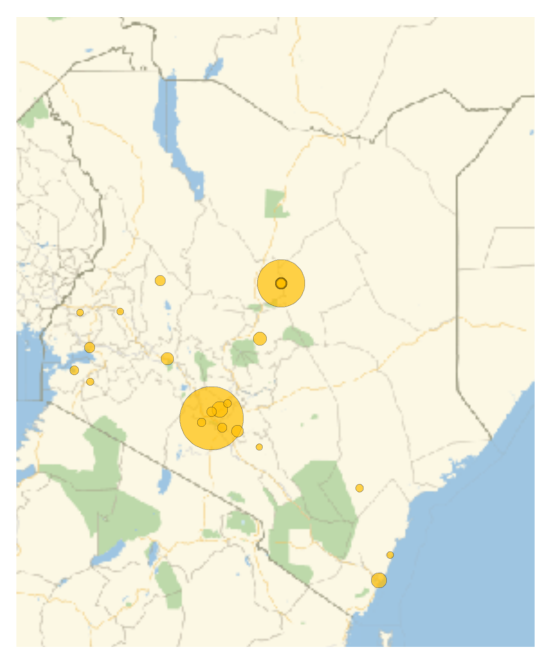
\includegraphics
[width=0.30\textwidth]{Kenya_density.eps}} 
\caption{Tweet distribution and densities in Canada and Kenya}
\end{figure}

Finally and most importantly, the populations of each country are prolific users of Twitter. In Canada there are over 7 million monthly active users on Twitter (Statista, 2017). In Kenya, there are an estimated 700 thousand monthly active users (Kemibaro, 2014). This means that Twitter provides an easy way of surveying the political moods of large sections of the Canadian and Kenyan populations. Figure 1 shows the distribution and concentration of the analyzed tweets, which follow the major population centers of each country. 

%get the peripheral data: G, S, GDP, Crime data. 

%cost associated with created a tweet 

%How do you quantify that level of complaining 

%How do we deal with re-tweets 

\section*{Data and Estimation}   

Summary statistics from the regular expression analysis are presented in Table 1. These are tweets that are explicitly about political issues of Canada or Kenya. During the period of analysis we observed 73,511 unique tweets from Canada and 37,603 from Kenya. As expected most tweets contained only a single regular expression. 

\begin{table}[]
\begin{spacing}{1}
\centering
\begin{tabular}{lcc}
\toprule
\multicolumn{1}{l}{} & \multicolumn{1}{l}{\textbf{Canada}} & \multicolumn{1}{l}{\textbf{Kenya}} \\ \hline
\textit{N} & 73,511 & 37,603 \\
Mean $\hat{d_{i,t}}$ & 1.48 & 4.74 \\
Std. dev. $\hat{d_{i,t}}$ & 0.86 & 0.76 \\
Mode $\hat{d_{i,t}}$ & 1 & 5 \\
Max $\hat{d_{i,t}}$ & 12 & 10 \\
& & \\
Mean $\hat{D_t}$ & 12,123.78 & 19,816.89 \\
Std. dev. $\hat{D_t}$ & 10,494.53 & 30,713.60 \\
\hline
\end{tabular}
\caption{Twitter Data Summary Statistics}
\end{spacing}
\end{table}

In nominal terms, there were more Canadian tweets expressing dissent than Kenyan. This result is likely because Canada has monthly active user population roughly ten times greater than Kenya. However, the interesting result is that even though there were more Canadian tweets, on average each individual Canadian tweet expressed less dissent than in Kenya. Average individual dissent in Canada was 1.48 compared to 4.74 in Kenya. 

Figure 2 shows the summed weekly estimated dissent levels for low(1-2), medium(3-5), and high(6+) dissent tweets and Figure 3 shows the combined total $\hat{D_t}$ for each country. Figures 2 and 3 show that even though there were less tweets from Kenya, on average there is a higher level of dissent in Kenya than Canada. Table 2 shows results from a Mann-Whitney U test and a Kolmogorov-Smirnov test that further indicate the presence of fundamental differences in dissent levels between the two countries. Given Kenya's previously stated issues with respect to corruption and political violence this makes sense. 

\begin{figure}[htb]
\centering 
\subfigure{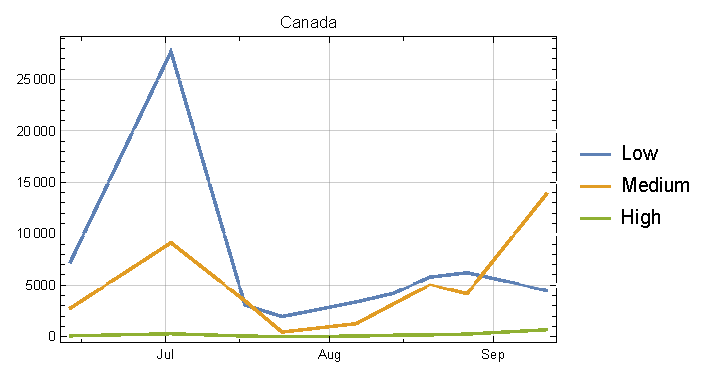
\includegraphics
[width=0.45\textwidth]{Canada_Dissent.eps}}
\subfigure{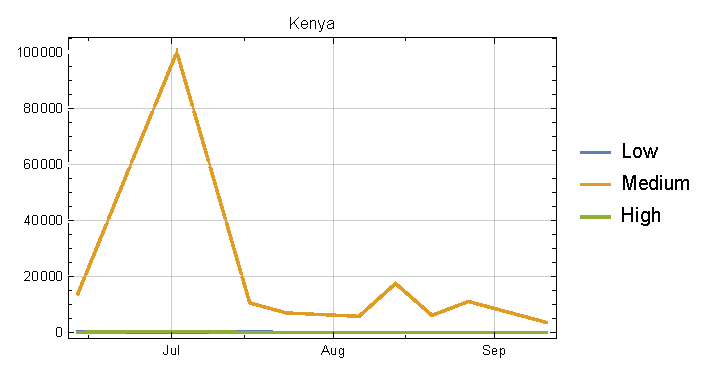
\includegraphics
[width=0.45\textwidth]{Kenya_Dissent.eps}} 
\caption{Weekly Dissent levels in Canada and Kenya}
\end{figure}

\begin{figure}[htb]
\centering 
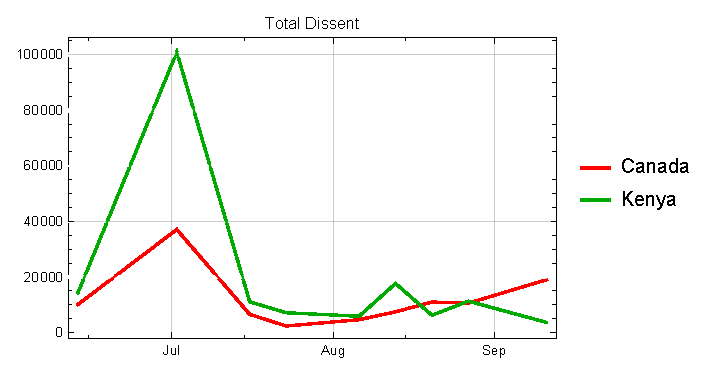
\includegraphics
[width=0.45\textwidth]{Total_Dissent.eps} 
\caption{Weekly Total Dissent levels in Canada and Kenya}
\end{figure}

\begin{table}[]
\begin{spacing}{1}
\centering
\begin{tabular}{ll}
\toprule
\multicolumn{2}{l}{Mann-Whitney U Test} \\
\multicolumn{2}{c}{P-value 0.000} \\
\multicolumn{2}{l}{Kolmogoro-Smirnov Test} \\
\multicolumn{2}{c}{P-value 0.000} \\ \hline
 
\end{tabular}
\caption{Statistical Tests}
\end{spacing}
\end{table}

Note that these results only accounts for those that expressed some form of dissent online ($\hat{d_{i,t}}>0$. Recall that Canada has 7 million active users on Twitter and Kenya 700 thousand. We did not detect dissent from most users in each country ($\hat{d_{i,t}}=0$). Roughly 1\% of Canadian Twitter users expressed some level of dissent during this period, while 5\% of Kenyan Twitter users did. The take away is that relative to their user populations, more Kenyans expressed dissent and at higher levels than Canadians.      

A possible reason we see more dissent in Kenya is that 2016 was a presidential election year. Elections have a tendency to highlight the short comings of the ruling regime, potentially increasing the level of dissent in a country. Given Kenya's past history with election violence, tensions were likely very high and observed this in Twitter.  



%As a robustness check and to ensure that the results in Figure 3 are not a product of the linear weighting of the regular expression scores, monotonic transformations were applied to the regular expression scores. Figure 4 again shows total dissent in Canada and Kenya but the results transformed through logarithmic, squared, and exponential functions. The previous results hold in all three cases, there is consistently more dissent in Kenya than Canada.  

%\begin{figure}[htb]
%\centering 
%\subfigure{\includegraphics
%[width=0.45\textwidth]{MonoLog.eps}}
%\subfigure{\includegraphics
%[width=0.45\textwidth]{MonoSqr.eps}} 
%\subfigure{\includegraphics
%[width=0.45\textwidth]{MonoExp.eps}}
%\caption{Monotonic Transformations of Total Dissent}
%\end{figure}

%\subsubsection*{Brexit}

Another interesting result of our analysis can be seen in Figures 2 and 3. Towards the end of June, there is a massive spike in dissent for both countries. Examination of news articles in each country during this period reveals no significant events that would explain the spike. However, broadening the scope to the world level does uncover an explanatory event: Brexit. 

\begin{figure}[htb]
\centering 
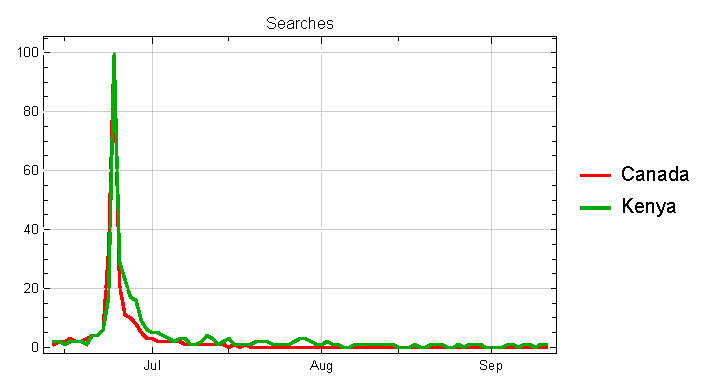
\includegraphics
[width=0.45\textwidth]{Brexit.eps} 
\caption{Daily Internet Searches for `Brexit' in Canada and Kenya}
\end{figure}

The UK referendum on whether or not to continue membership in the European Union, colloquially known as `Brexit', occurred on June 23, 2016. The slight skew towards the beginning of July on the time line is a result of scaling the original time series from daily to weekly. Search history for `Brexit' from Google Trends (Figure 4) for each country, confirms that citizens from each country were interested in the events of Brexit. Given that Canada and Kenya were UK colonies and each maintains friendly relationships with the UK, it's logical that UK politics would be of interest to citizens of Canada and Kenya. However, that relationship alone does not explain why we see a spike in dissent in each after Brexit. 

A possible explanation is that the events of Brexit may have encouraged people to discuss their own country's issues. Since people use Twitter as a news source (Smith and Wooten, 2013; Twitter, 2016), it is entirely plausible that they logged on to Twitter to see/discuss what was going on with Brexit and then stayed to discuss political events relevant to their own country. This reveals an unexpected sensitivity to outside large scale events this type of analysis might have. However, as we know from the Arab Spring (The Economist, 2016), events in one country can often inspire events in another. This is especially true when it comes to issues of political stability. Given that the regular expressions used for scoring were coded to explicitly capture exclusively Canadian and Kenyan issues, this is the most likely explanation.    

%Include a pie chart breaking down the percentage of issues that people are upset about: Politicians, economic issues, quality of life? 






\subsection*{Estimating Political Stability}

\begin{table}[]
\begin{spacing}{1}
\centering
\begin{tabular}{lcc}
\toprule	
 & \textbf{Canada} & \textbf{Kenya} \\ \hline
\begin{tabular}[c]{@{}l@{}}2016 Civil Expenditures\\ (2010 US\$)\end{tabular} & 368,837,027,606 & 6,823,643,525 \\
\begin{tabular}[c]{@{}l@{}}2016 Military Expenditures\\ (2010 US\$)\end{tabular} & 18,068,962,843 & 732,694,153 \\
$\alpha$ & .414 & .759 \\
$\gamma$ & .586 & .241 \\ \hline
\multicolumn{3}{l}{Source: World Bank}
\end{tabular}
\caption{Estimation Values}
\end{spacing}
\end{table}

Table 3 shows the 2016 values of government civil and military expenditures from each country along with their estimated preferences for each. Using the functional form provided by Equation (2), we can obtain a weighted weekly estimates of political stability. 

\begin{figure}[htb]
\centering 
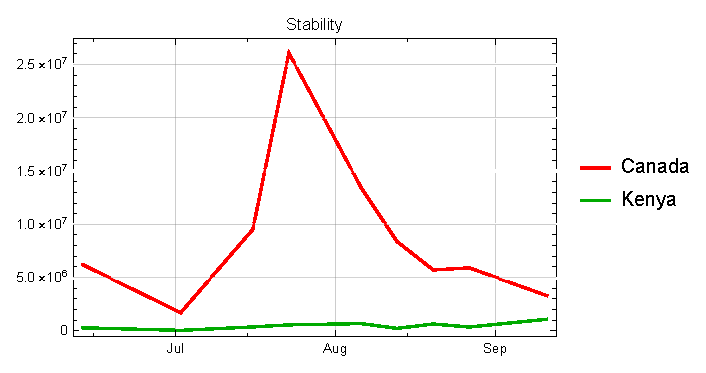
\includegraphics
[width=0.45\textwidth]{Political_Stability.eps} 
\caption{Weekly Nominal Estimated Political Stability in Canada and Kenya}
\end{figure}

Figure 5 shows our nominal estimates of political stability for Canada and Kenya. To get estimates of political stability each country relative to one another, dissent estimates are rescaled based on active monthly user population. Government expenditures are also rescaled to control for population differences. The normalized scaled estimates of political stability are shown in Figure 6.    

\begin{figure}[htb]
\centering 
\includegraphics
[width=0.45\textwidth]{Scaled_PS.eps} 
\caption{Weekly Scaled Estimated Political Stability in Canada and Kenya}
\end{figure}

Again, the results adhere to a priori expectations. Controlling for population differences only magnifies the findings. Canada appears to be more politically stable than Kenya. This means that Canada is likely more resilient to potential exogenous shocks (recession, terrorist attacks, natural disaster, health crisis, etc) than Kenya would be to the same shock. Canada's developed economy, efficient government, and strong civil society likely factor heavily in this result. While showing that Canada is more politically stable than Kenya may seem like an obvious result, it is nonetheless important. The disparity between the estimates of the two signifies that this is a valid method of cross country analysis.


\section*{Conclusion}

%What we did
This paper has presented a new method of estimating public dissent and political stability. By collecting tweets expressing dissent against the government and weighting with government and military expenditures, we were able to obtain estimates of political stability for Canada and Kenya. Our estimates show that Canada is likely more politically stable than Kenya. Our results are in line with other methods, highlighting the verifiability of this process. While this paper used data from Twitter as its basis, the methodology could easily be employed to other similarly structured social media platform one has access too.    

%Why it's important

Knowing what countries are potentially in crisis is important for several reasons. First, being able to intervene before a country falls apart is far easier than trying to reassemble the broken pieces. Second, these failed states often become havens for criminals, terrorists, and other misanthropes. Third, instability in one country has a nasty habit of leaking beyond its borders. The failed state of Somalia is an unfortunate testament to all three. As the whole world becomes more integrated knowing where crisis may emerge becomes ever more critical. 

%Criticisms 

As important as this research is, it is not impervious to criticism. A primary issue with this method of estimating political stability is that it is highly dependent upon the social media population. The smaller the population using Twitter in a country, the less useful this estimate will be. However, growing the user base, especially in developing countries, is a strategic goal of Twitter Inc (Twitter, 2016). The steady rise in smart phone usage across the world (Poushter, 2016) should aid Twitter's market penetration. 

Another issue is that some governments are manipulating social media for their own benefit (King, 2016). This is a concern but one that is likely overstated. Only a few countries in the world have both the desire and the means to negatively affect social media platforms. Furthermore, a social media company's entire business is predicated upon its ability to maintain users. If consumers do not feel that they are getting an honest experience on a platform, they will go elsewhere. Thus it becomes the goal of multibillion dollar firms to counter the machinations of rogue states. 

The final critique of using social media data is that we have selection bias because these platforms tend to have a younger user base. This is certainly the case with Twitter users in Canada (Insights West, 2016) and Kenya (Simon et al., 2014), where the average Twitter user is in their twenties. However, Rothchild (2015) shows that a properly statistically weighted non-representative sample can still be effective for poll forecasting. Additionally, this potential bias may even be an asset that enhances our measure. The demographic group most likely to use social media, the young, are also the most likely to advocate for large scale political change. Thus by forming the basis of our measure on dissent on social media, we're actually able to account for the group most likely to take to the streets.
    
The goal of this paper is not to replace traditional means of measuring political stability. Instead, it is meant as an enhancement incorporating societal and technological changes to increase the accuracy of estimates. Substantive expertise is still necessary to identify key issues, knowing what expressions people use for expressing dissent, and how to properly judge the validity of those statements. However, using this framework would help reduce the subjective nature of interpreting political stability. 


\end{spacing}

\pagebreak

\bibliographystyle{chicago}
\bibliography{Twitter_Bibli}

\nocite{*}



\end{document}	

